\documentclass{report}
\usepackage[T1]{fontenc} % Fontes T1
\usepackage[utf8]{inputenc} % Input UTF8
\usepackage[backend=biber, style=ieee]{biblatex} % para usar bibliografia
\usepackage{csquotes}
\usepackage[portuguese]{babel} %Usar língua portuguesa
\usepackage{blindtext} % Gerar texto automaticamente
\usepackage[printonlyused]{acronym}
\usepackage{hyperref} % para autoref
\usepackage{graphicx}
\usepackage{indentfirst}

\begin{document}

%%
% Definições
%
\def\titulo{Misturador de Músicas}
\def\data{15/06/2018}
\def\autores{André Alves, Daniel Correia, Pedro Almeida, Pedro Valente}
\def\autorescontactos{(88811) andr.alves@ua.pt, (88753) dcorreia@ua.pt,\\
 (89205) pedro22@ua.pt, (88858)pedro.valente@ua.pt}
\def\departamento{Departamento de Electrónica, Telecomunicações e Informática}
\def\empresa{Universidade De Aveiro}
\def\logotipo{img/ua.pdf}
%

%%%%%% CAPA %%%%%%
%
\begin{titlepage}

\begin{center}
%
\vspace*{50mm}
%
{\Huge \titulo}\\ 
%
\vspace{10mm}
%
{\Large \empresa}\\
%
\vspace{10mm}
%
{\LARGE \autores}\\ 
%
\vspace{30mm}
%
\begin{figure}[h]
\center
\includegraphics{\logotipo}
\end{figure}
%
\vspace{30mm}
\end{center}
%

\end{titlepage}

%%  Página de Título %%
\title{%
{\Huge\textbf{\titulo}}\\
{\Large \departamento\\ \empresa}
}
%
\author{%
    \autores \\
    \autorescontactos
}
%
\date{\data}
%
\maketitle

\pagenumbering{arabic}

\chapter{Introdução}
\label{chap.introducao}
O objetivo do projeto é a criação de um sistema que permita criar músicas através da
composição de pedaços de música. O projeto funciona a partir de um servidor do XCOA.
O sistema é composto por vários componentes, componentes estes que são:
\begin{itemize}
	\item Interface Web
	\item Aplicação Web
	\item Persistência
	\item Gerador de Músicas
\end{itemize}	

A Interface Web (\autoref{chap.interface}) é composta por quatro páginas HTML cada uma com 
um propósito prório a explicar mais à frente.

A página Início é uma pequena página inicial na qual o utilizador poderá ver 
aquilo que pode fazer neste site, assim como algumas informações sobre os autores e o local onde o projeto foi desenvolvido.
	
As Aplicações Web consistem num programa python que serve conteúdos estáticos, 
esta parte do trabalho serve como ponte para todos os outros componentes, para além disto tem também objetivos próprios a ser 
explicados mais à frente na \autoref{chap.aplicacao}.

A parte da Persistência consiste numa base de dados relacional e obtenção de dados da mesma, 
tudo isto será depois utilizado pela parte das Aplicações Web para registar as músicas criadas, os excertos que existem e os 
votos de cada um dos utilizadores, explicado em maior detalhe em \autoref{chap.persistencia}.

A parte do Gerador de Música é composta por uma grelha na qual o utilizador poderá escolher o excerto e onde poderia adicionar efeitos e alterar o volume. Se a geração tivesse tido sucesso, a música iria ser escrita no sistema de
ficheiros(base de dados). Este componente deveria suportar 3 efeitos a aplicar no momento da geração
da música, tudo isto será mais aprofundado na \autoref{chap.gerador}.

\newpage
\chapter{Desenvolvimento}
\label{chap.desenvolvimento}

Neste capítulo vamos passar a explicar o código que fizemos de acordo com aqueles que eram os objetivos e o que ficou por fazer 
em cada uma das partes.
	
\section{Interface Web}
\label{chap.interface}
..............
\newpage
\section{Aplicação Web}
\label{chap.aplicacao}
................
\newpage
\section{Persistência}
\label{chap.persistencia}
Este projeto contém uma base de dados que recorre à utilização de três tabelas, todas as tabelas são alteradas consoante as funções de Python existentes no resto do projeto.
Tabelas estas que vão de seguida enviar os dados para as páginas HTML através de JavaScript.
A tabela das samples serve para guardar todos os excertos que colocámos disponíveis.
Esta tabela tem como componentes:
	\begin{itemize}
		\item Name   -> do tipo TEXT
		\item Date   -> do tipo TEXT
		\item ID     -> do tipo TEXT
		\item Length -> do tipo INTEGER
		\item Uses   -> do tipo INTEGER
	\end{itemize}


A tabela das músicas serve para guardar todas as músicas criadas pelos utilizadores Misturador, esta tabela deverá conter apenas uma amostra exemplar, isto porque o nosso misturador não funcionava pelo que esta tabela não irá receber dados.
Esta tabela terá também uma contagem de votos assim como o autor de cada uma das músicas.
Esta tabela tem como componentes:
	\begin{itemize}
		\item Name -> do tipo TEXT
		\item Date -> do tipo TEXT
		\item ID -> do tipo TEXT
		\item Length -> do tipo INTEGER
		\item Uses -> do tipo INTEGER
		\item Votes -> do tipo INTEGER
		\item Author -> do tipo TEXT
	\end{itemize}

A tabela dos votos irá ter a função de guardar os votos que são inseridos em cada uma das músicas, cada utilizador apenas pode ter um voto numa música(pode votar 1, -1 ou deixar 0 se se quiser manter imparcial).
É permitido ao utilizador alterar o seu voto.
Esta tabela tem como componentes:
	\begin{itemize}
		\item Email -> TEXT
		\item sID -> TEXT
		\item Points -> INTEGER
	\end{itemize}

\newpage
\section{Gerador de Músicas}
\label{chap.gerador}
...................
\newpage
\chapter{Resultados}
\label{resultados}

\section{Demonstração do funcionamento dos Votos}
\begin{figure} [h]
	\centering
	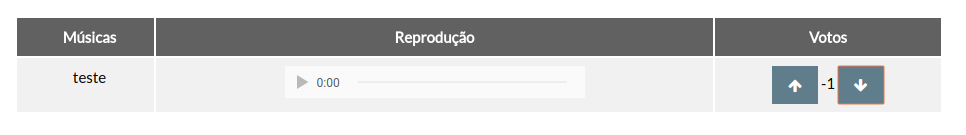
\includegraphics [scale = 0.4] {img/votos-1}
	\caption{Resultado dos votos para: -1}
\end{figure}

\begin{figure} [h]
	\centering
	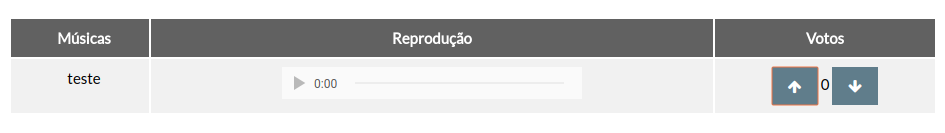
\includegraphics [scale = 0.4] {img/votos0}
	\caption{Resultado dos votos para: 0}
\end{figure}

\begin{figure} [h]
	\centering
	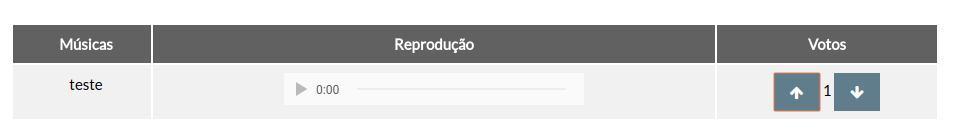
\includegraphics [scale = 0.4] {img/votos1}
	\caption{Resultado dos votos para: 1}
\end{figure}

\section{Demonstração do funcionamento da página Excertos}
\begin{figure} [h]
	\centering
	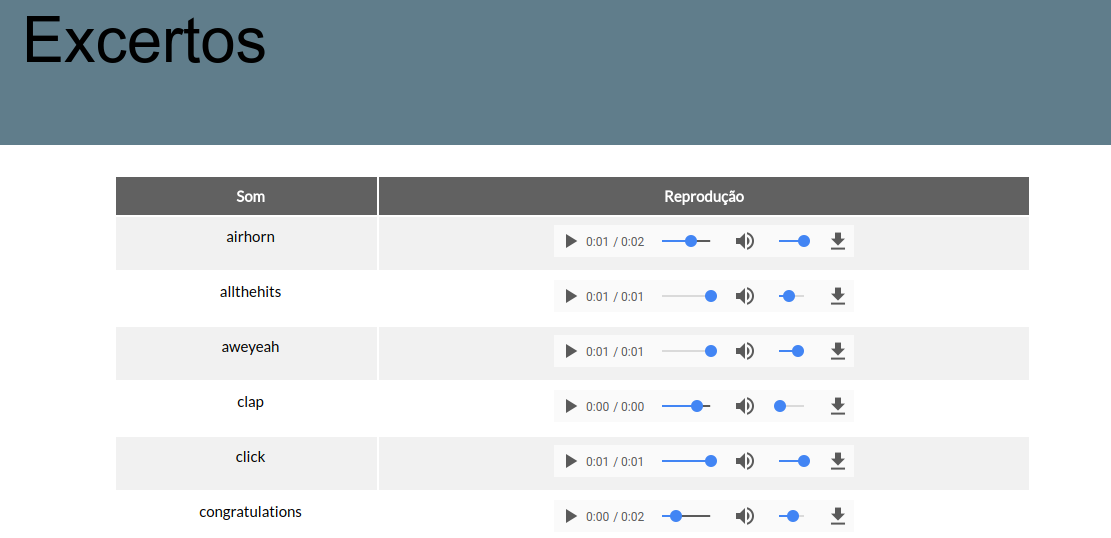
\includegraphics [scale = 0.3] {img/excertos}
	\caption{Funcionamento de todos os componentes da página excertos}
\end{figure}

\newpage
\section{Demonstração do funcionamento da Base de Dados}
\begin{figure} [h]
	\centering
	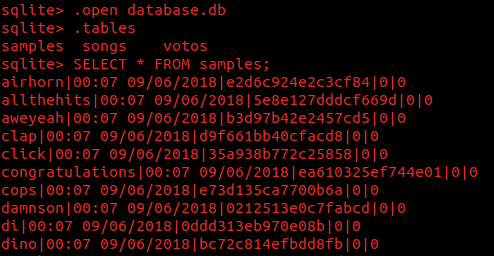
\includegraphics [scale = 0.4] {img/samples}
	\caption{Funcionamento da tabela samples}
\end{figure}

\begin{figure} [h]
	\centering
	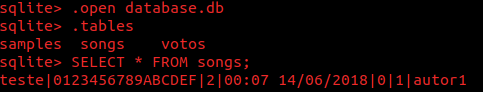
\includegraphics [scale = 0.5] {img/songs}
	\caption{Funcionamento da tabela songs}
\end{figure}

\begin{figure} [h]
	\centering
	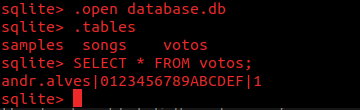
\includegraphics [scale = 0.5] {img/votos}
	\caption{Funcionamento da tabela votos}
\end{figure}

\newpage	 
\chapter{Conclusões Finais}
\label{chap.conclusao}
	Com este projeto de gerador de músicas foi possível consolidar os conhecimentos 
	adquiridos em aulas pois foi necessário tudo o que foi realizado ao longo semestre. 
	
	Infelizmente, o projeto não está completamente funcional. Ainda assim, com o que foi feito, mudou a forma como os 
	elementos do grupo veem as aplicações como esta de gerador de músicas, todo o trabalho que está por detrás do que é 
	apresentado ao utilizador.  

 \newpage
\chapter{Contribuições dos autores}
\label{contribuições}

\noindent
André Alves - 25\% \\
Daniel Correia - 25\% \\
Pedro Almeida - 25\% \\
Pedro Valente - 25\% 


\end{document}